\section{Introduction}
\label{sec:introduction}
% Faithful translation of the existing Chinese introduction.
Graph analysis under local differential privacy (LDP) has become an important research direction in graph data analytics.
These techniques aim to enable an untrusted server in a distributed setting to perform graph-structure statistics and analysis without exposing users' private information, including private edges or adjacency information.
Existing studies have developed basic graph analysis operators for node degrees and subgraph counting~\cite{imola2021locally,Ye2022}.
However, existing LDP graph analysis operators primarily target node-level scalar statistics or global structural counts, rather than the \textbf{triangle degree distribution (TDD)}. %
Triangle degree counts the triangles containing a node; the TDD counts nodes with each triangle degree.
Compared with node degrees or global triangle counts, which reflect local connectivity or overall triangle abundance, TDD preserves information on local triangle participation and its heterogeneity across nodes~\cite{becchetti2008local,antunes2021sampling}.
TDD therefore serves as an important structural statistic for graphlet-based network comparison~\cite{LDPGDDPrzulj2007,hayes2013graphlet} and as an input for graph generation~\cite{zahirnia2023neural}.
% TDD therefore provides a useful structural descriptor for network comparison and the characterization and modeling of clustered network structures~\cite{LDPGDDPrzulj2007,pham2024clustering}.


% Graph analysis under local differential privacy (LDP) has become an important research direction in graph data analytics.
% These techniques aim to enable an untrusted server in a distributed setting to perform graph-structure statistics and analysis without exposing users' private information, including private edges or adjacency information.
% Existing studies have developed basic graph analysis operators for node degrees, triangle counting, and subgraph counting~\cite{imola2021locally,Ye2022}.
% However, existing LDP graph analysis operators primarily target individual scalar statistics or a small number of global structural counts, and cannot yet support operators such as the \textbf{triangle degree distribution (TDD)}.
% TDD characterizes the frequency distribution of the numbers of higher-order graphlets in which nodes or edges participate.
% Compared with scalar statistics such as node degrees or global triangle counts, which reflect only local connectivity or overall closure, TDD preserves richer local structure and its heterogeneity across nodes~\cite{faloutsos1999power,tsourakakis2008fast,sphICDM}.
% TDD therefore offers greater structural expressiveness and supports a broader range of applications, including network comparison, motif identification, anomalous topology detection, and biological and financial network analysis~\cite{motifs,subgraphTopolgy,LDPTDDPrzulj2007,wegner2018identifying,yoon2023graphlets,elliott2019anomaly}.

Existing techniques cannot adequately support an  applicable TDD operator under LDP, as illustrated in Fig.~\ref{fig:tdd-motivation}\subref{fig:tdd-limitation}.
As with existing LDP operators, implementing a TDD operator requires both local randomized reporting and server-side aggregation and estimation~\cite{LDPGDDWang2017,imola2021locally}, and its central difficulties arise in both stages.
First, during local randomized reporting, users must randomize and report the private quantity to be aggregated, namely their triangle degree.
However, in the TDD task under distributed privacy constraints, each user does not know this value in advance.
% Using existing LDP techniques, \textbf{estimating this unknown scalar introduces additional error}, because each user must perform an LDP-compliant aggregation and recovery procedure to obtain it.
Using existing LDP techniques, \textbf{estimating this locally unknown scalar introduces additional error}, as it requires inferring triangle degrees from noisy information about edges.
Second, during server-side aggregation and estimation, the TDD operator must estimate a histogram of triangle degrees rather than a single scalar statistic. %the complete distribution of graphlet degrees, typically represented as a histogram, rather than a simple scalar statistic.
Directly applying existing LDP techniques to \textbf{estimate this high-dimensional distribution further amplifies the additional error introduced in the preceding stage}.
% Taking \draftplaceholder{} as an example, the procedure first \draftplaceholder{} and then assigns nodes to the corresponding histogram bins according to their locally randomized reported values.
For example, LDPGraph estimates triangle degrees from privatized graph reports~\cite{dong2026ldpgraph}.
A direct TDD adaptation would discretely bin these estimates.
Unlike linear aggregation tasks such as global triangle counting, where positive and negative errors may cancel in summation, such binning can shift nodes between bins and distort the histogram, especially under tighter privacy budgets.
% Unlike linear aggregation tasks such as global triangle counting, however, TDD requires discrete binning before aggregation.
% Unlike global triangle counting, where positive and negative numerical errors may cancel during summation, such binning can move nodes between histogram bins, distorting their frequencies.
% Consequently, noise introduced by the LDP mechanism cannot cancel out through aggregation into a single scalar statistic, instead, it is distributed across histogram bins. %and manifests as mass migration between bins.
% The estimation error in the previously unknown scalar is thus further transformed into additional distributional distortion.
% In particular, under stronger privacy constraints, greater uncertainty in recovery further increases such cross-bin errors.
%the probability of nodes crossing bin boundaries, ultimately producing substantial TDD distortion.

% \begin{figure}[t]
%   \centering
%   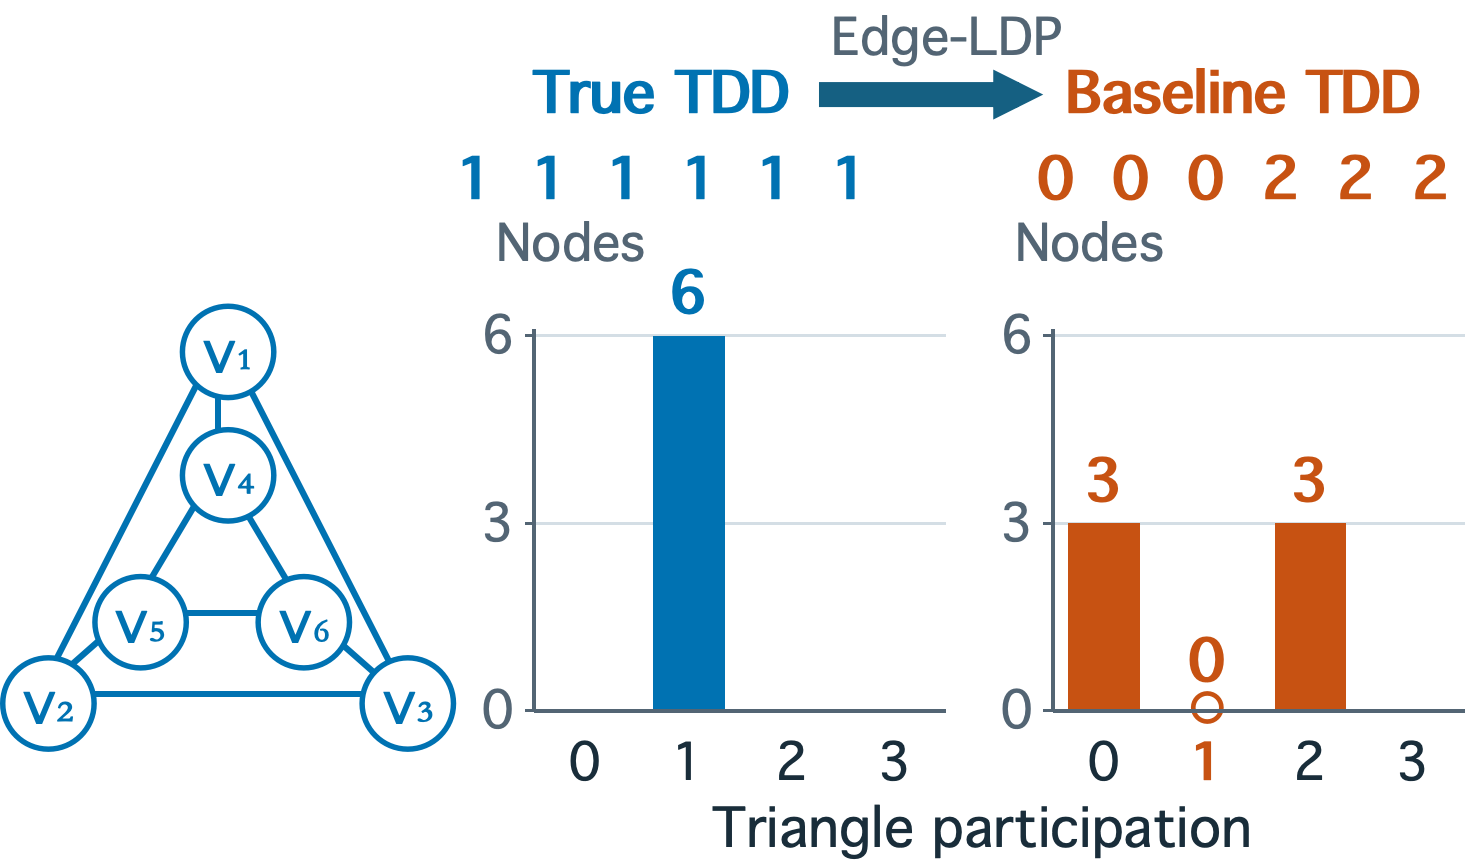
\includegraphics[trim=0mm 0mm 0mm 0mm,clip,width=\linewidth]{icde_sections/limitation.png}
%   \caption{Limitations of baseline composed by existing LDP operators.}
%   \label{fig:limitation}
% \end{figure}

% \begin{figure}[t]
%   \centering
%   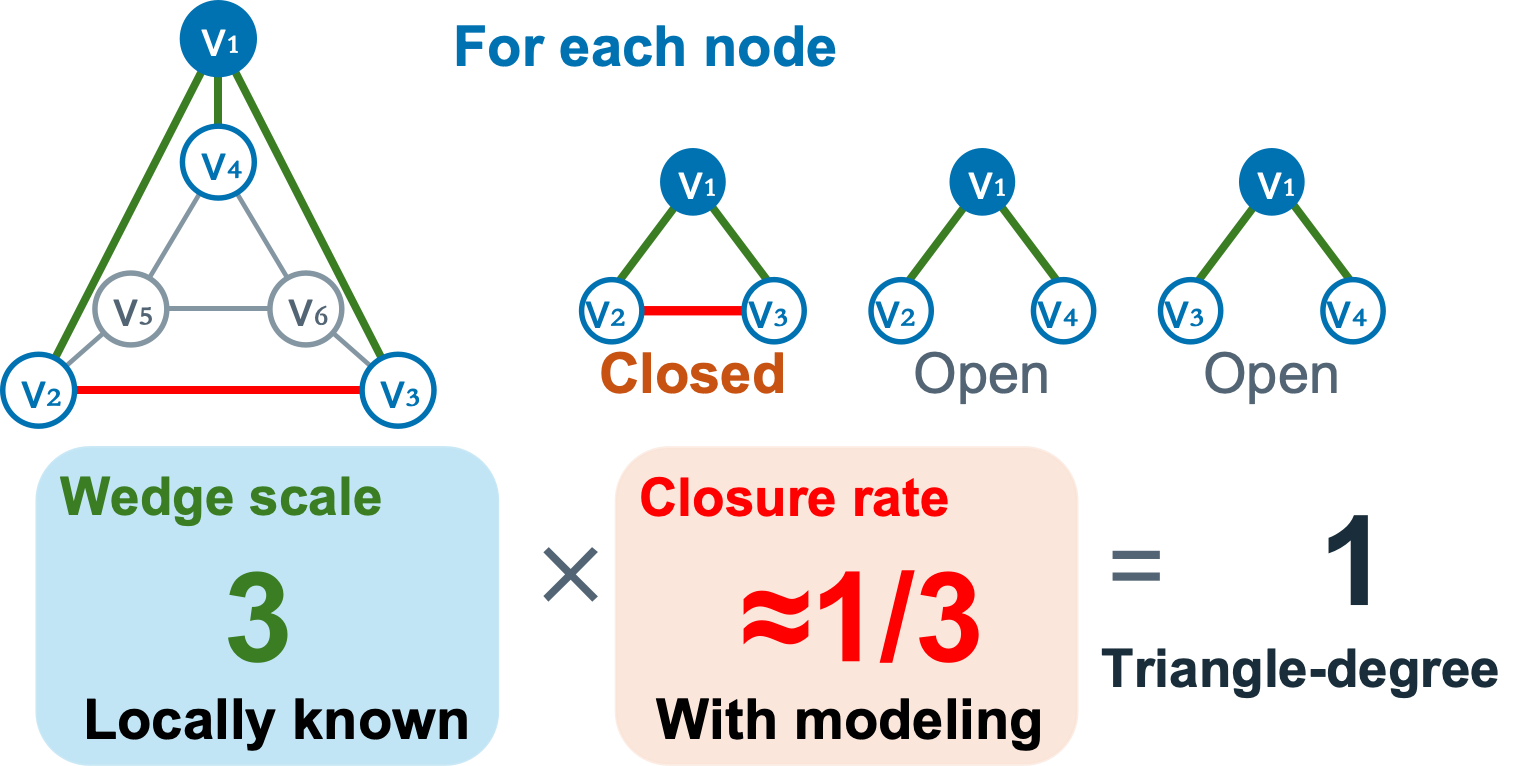
\includegraphics[trim=0mm 0mm 0mm 0mm,clip,width=\linewidth]{icde_sections/basic idea.png}
%   \caption{Basic idea of PrivTDD.}
%   \label{fig:basic_idea}
% \end{figure}


\begin{figure}[t]
    \centering
    \subfloat[Limitation of existing techniques]{
        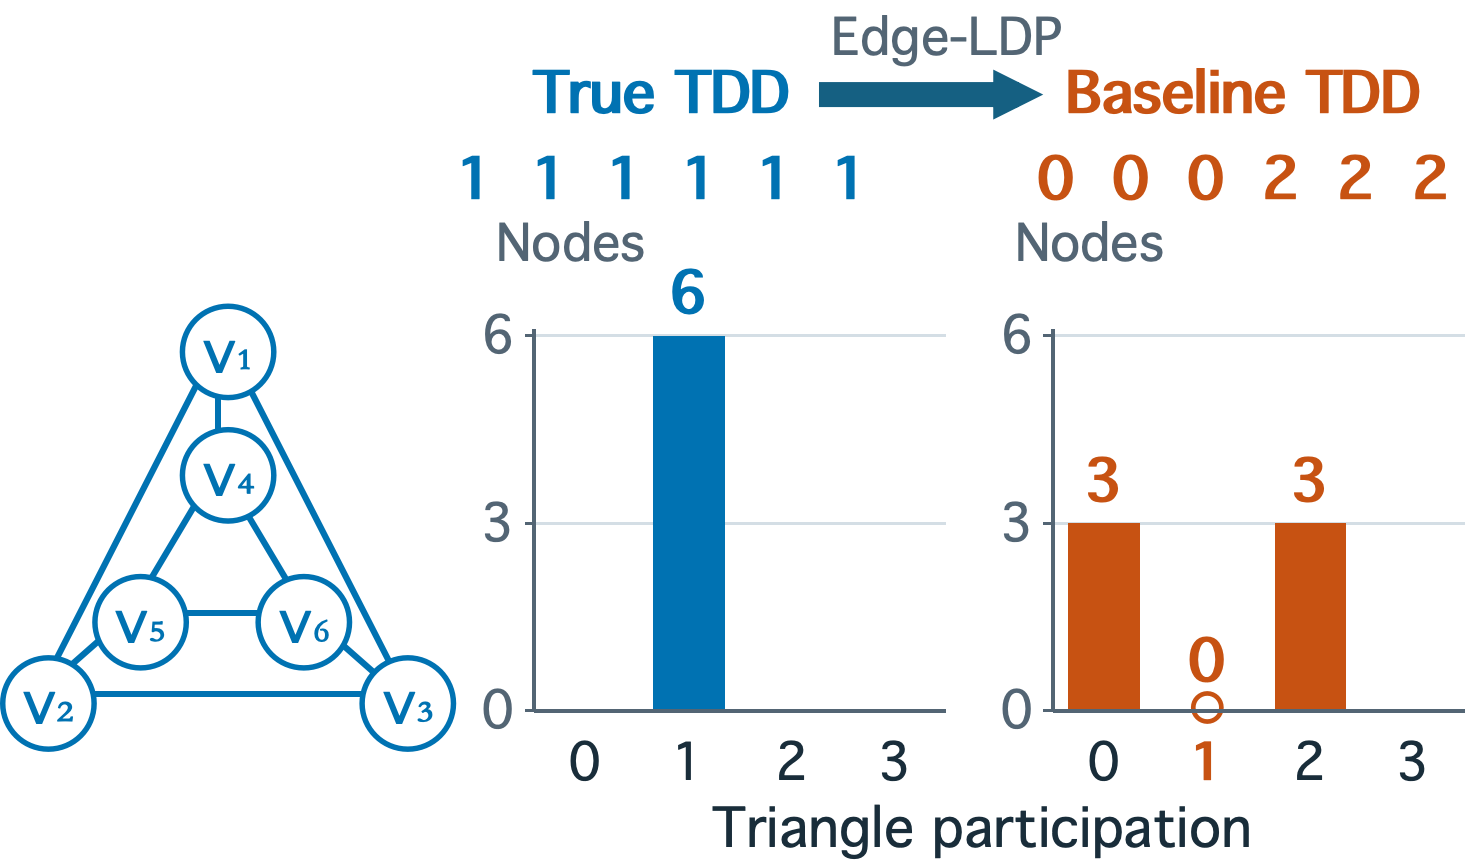
\includegraphics[width=0.45\columnwidth]{icde_sections/limitation.png}
        \label{fig:tdd-limitation}
    }
    \hfill
    \subfloat[Basic idea]{
        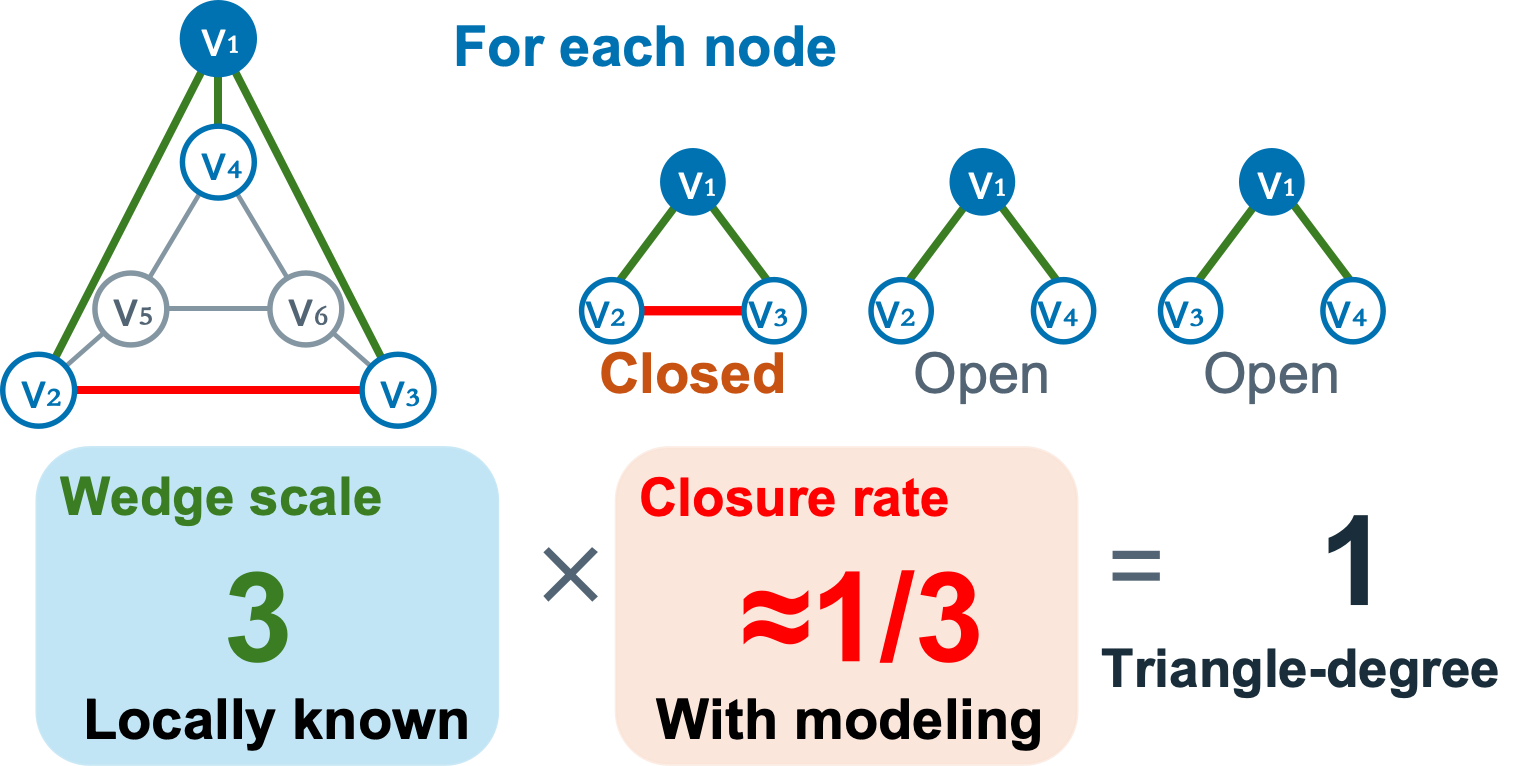
\includegraphics[width=0.45\columnwidth]{icde_sections/basic idea.png}
        \label{fig:tdd-basic-idea}
    }
    \caption{(a)  Existing techniques cannot support an applicable TDD operator under LDP, since binning noisy triangle-degree estimates can distort the TDD despite an accurate global triangle count.
    (b) Our basic idea is to decompose triangle-degree estimation into wedge-count and closure-rate (red) estimation.}
    \label{fig:tdd-motivation}%todo
\end{figure}


This paper proposes the first TDD operator under LDP, \textbf{PrivTDD}.
Its central idea is to transform the complex TDD estimation operator into a combination of two simpler estimation operators.
Specifically, instead of computing the TDD by assigning triangle degree values to different histogram bins, the method decomposes direct TDD estimation into modeling the distributions of \textbf{wedge counts} and \textbf{closure rates} (as illustrated in Fig.~\ref{fig:tdd-motivation}\subref{fig:tdd-basic-idea}).
A node has one wedge per neighbor pair; its closure rate is the fraction connected. This decomposition provides two benefits.
First, and more directly, estimating the wedge-count distribution introduces little error.
Although this remains a high-dimensional histogram estimation task, it only aggregates wedge counts, which users already know, rather than triangle degrees, which they do not.
The resulting error is therefore much smaller than the error involved in estimating an unknown quantity, avoiding the additional two-stage error amplification described above.
The second benefit is more subtle.
Estimating closure rates through LDP alone does not yield more accurate estimates, because the closure-rate distribution still concerns quantities unknown to users.
However, modeling allows PrivTDD to estimate the closure-rate distribution by pooling information from different nodes' private reports.
For example, consider an extreme case in which all nodes with wedges in a network have the same closure rate.
The closure-rate distribution is then determined by a single parameter; under this distributional model, we need only estimate that scalar parameter from private reports to obtain a lower-variance estimate.
For general settings, however, making distribution estimation more accurate through modeling requires addressing the following two challenges.

The first challenge is how to \textbf{construct informative structural references} for triangle degrees from limited private statistics.
The available reports do not reliably reveal how often neighbor pairs connect or how these connections depend on one another. Node degrees reveal only wedge counts.
We use two structural models to predict triangle-degree distributions at each node degree. The models share edge probabilities fitted from privatized degree reports.
A $\beta$-model~\cite{chatterjee2011random} captures the degree-driven baseline under independent edges, while a hidden-geometric model~\cite{serrano2008selfsimilarity} introduces latent proximity to represent local clustering that degrees alone cannot encode. 
These reference distributions guide correction.

% The first challenge is how to construct structural models that assist in recovering the triangle-participation distribution.
% Closure information inferred from privatized relational reports is noisy, while node degrees only determine wedge scales, not how neighbors connect.
% To address this challenge, we consider two factors influencing triangle participation: degree heterogeneity and local clustering.
% We therefore construct two complementary structural references based on private degree information.
% A $\beta$-model\cite{chatterjee2011random} characterizes participation under degree-driven independent edges, while a hidden-geometric model\cite{serrano2008selfsimilarity} introduces latent proximity to capture local clustering dependencies.
% These references jointly guide subsequent distribution correction.
% The first challenge is how to construct structural models that assist in recovering the triangle-participation distribution.
% Triangle participation in a network is influenced by both degree heterogeneity and local clustering.
% We construct two complementary structural reference distributions based on private degree information.
% First, we use a $\beta$-model that computes edge probabilities from degrees to construct a triangle-participation distribution under an edge-independence assumption.
% Second, because independent edges cannot capture local clustering dependencies among neighbors, we draw on hidden geometric network models and introduce the influence of latent node positions on edge formation to construct a triangle-participation distribution that accounts for local clustering.
% The outputs of these two structural models jointly provide a basis for subsequent distribution correction.




% The second challenge is how to use structural models to refine the network's distribution.
% Structural model outputs may deviate from the real network, while the true TDD is unavailable, making it impossible to choose correction strengths directly against the ground truth.
% We therefore use learnable parameters to control correction strengths.
% For the participation distributions obtained with different parameters, we compute the corresponding noisy-report distributions according to the known LDP reporting mechanism, and learn the parameters from the likelihood of the observed reports under those distributions.
% Moreover, because each node reports independently under LDP, recovering parameters independently for every node would introduce too many parameters, whereas treating the entire curve as a single recovery unit would be insufficiently accurate.
% We therefore adopt a divide-and-conquer approach that decomposes distribution correction along two dimensions.
% First, we recover the correction piecewise.
% We partition the distribution into several regions along the range of triangle-participation counts and use a small number of shared parameters to control correction in each region.
% Nonnegativity and global total-mass conservation constraints ensure that these regions jointly form a valid complete distribution.
% Second, we further decompose each region's distribution into probability mass and within-region shape.
% Mass describes the total probability assigned to the region, while shape describes the relative allocation of that probability among participation counts within the region.
% We assign separate correction strengths to mass and shape, and jointly learn their parameters using the report-fitting objective described above to refine the entire network's distribution.
The second challenge is how to \textbf{adjust an initial triangle-degree distribution at each node degree using structural references}.
References can be inaccurate, and ground truth is unavailable for deciding how much to adjust.
We assess each adjustment by how well the resulting distribution explains the private reports.
Correcting each triangle-degree value at each node degree separately introduces too many parameters; a single correction cannot accommodate differences across count ranges.
We divide the count range into regions and adjust both their probabilities and the allocation within each region, using a few parameters shared across node degrees.
Finally, we update count probabilities using each node's reports and aggregate across node degrees to estimate the TDD.


% % Appended ending. Unavailable results remain xxx.
% After these corrections, PrivTDD performs one further posterior reweighting step using the existing private reports and obtains the final triangle-participation distribution through probabilistic aggregation.
% During this process, the server retains the support that each report provides for different candidate participation counts, rather than prematurely reducing each node to a point estimate and assigning it to a single bin.
% Finally, degree-conditioned participation distributions are combined using the recovered overall degree distribution as weights to obtain the complete TDD.
% Structural modeling, distribution correction, and final aggregation all operate on the released private reports and consume no additional privacy budget.

We conduct rigorous theoretical analysis and extensive empirical evaluation of PrivTDD.
We prove its edge privacy guarantee, bound the expected earth mover's distance (EMD) between the released and true TDDs, and derive a privacy budget allocation that minimizes the bound.
%The EMD bound matches the minimax rate under the assumptions in Section~\ref{sec:analysis}.
We compare PrivTDD with adapted triangle-counting and graph-synthesis baselines under consistent privacy accounting on four real-world networks, including Orkut with 3.07 million nodes and 117.2 million edges.
PrivTDD achieved the lowest mean EMD in 30 of 32 network--budget settings.
On DBLP at privacy budget $\varepsilon=2$, its mean EMD was 2.65 versus 28.24 for the best baseline, LDPGraph-T, a 90.6\% reduction.
Ablation studies examine structural modeling and report-driven correction. We also vary the region boundaries and measure how sampling neighbor pairs affects TDD estimation error.

Our contributions are summarized as follows:
\begin{itemize}

\item We investigate \textbf{triangle degree distribution (TDD) estimation under edge-local differential privacy (edge-LDP)}. %, where each node has access only to its own adjacency information.
We identify two limitations of directly combining private counting with histogram aggregation: triangle degrees are not locally available, and binning their noisy estimates can distort the target histogram.


\item We propose \textbf{PrivTDD}, which decomposes TDD estimation into the estimation of a \textbf{wedge-count distribution and closure-rate distributions}.
It constructs complementary $\beta$ and geometric structural references to capture degree heterogeneity and local clustering, learns regional mass and within-region shape corrections from private reports, and forms a TDD estimate through posterior reweighting and probabilistic aggregation.

\item We establish privacy  guarantees for PrivTDD and derive a budget allocation that minimizes the error bound.
Experiments on four real networks evaluate estimation accuracy, the contributions of the core designs, sensitivity to region boundaries, and accuracy under neighbor-pair sampling.
Artifacts are available at \url{https://github.com/Luna-iris/PrivTDD}.
\end{itemize}
